\documentclass[24pt, a0paper, portrait, margin=0mm, innermargin=15mm, blockverticalspace=15mm, colspace=15mm, subcolspace=-5mm]{tikzposter}
\tikzposterlatexaffectionproofoff



\usepackage{tabulary}
\usepackage{caption}
\usepackage{amsmath, amsthm, amssymb, units, dsfont}
\usepackage{sidecap}
\usepackage{enumerate}
\usepackage{xcolor}

\usepackage{mathtools, mathdots}
\usepackage{pgffor}
\usepackage{pdflscape}
\usepackage{afterpage}
\usepackage{chngcntr}
\usepackage{multirow}
\usepackage{tabulary}

\usepackage{listings}
\usepackage{color}

\usepackage{algorithm}
\usepackage{algorithmic}

\usepackage{breqn}
\usepackage{hyperref}

\usepackage{pgfkeys}

\usepackage{changepage}

\definecolor{darkgreen}{rgb}{0,0.6,0}
\definecolor{darkred}{rgb}{0.6,0,0}
\definecolor{darkblue}{rgb}{0,0,0.6}
\definecolor{darkgrey}{rgb}{0.3,0.3,0.3}
\definecolor{grey}{rgb}{0.6,0.6,0.6} %comment
\definecolor{lightgrey}{rgb}{0.92,0.92,0.92}
\definecolor{terminal}{rgb}{0.9,0.9,0.6}
\definecolor{cmd}{rgb}{0.8,0.8,0.98}
\lstset{ 
        basicstyle=\ttfamily,
%         language=Matlab,                                % choose the language of the code
%       basicstyle=10pt,                                % the size of the fonts that are used for the code
%         numbers=left,                                   % where to put the line-numbers
        keywordstyle=\color{darkblue},
        commentstyle=\color{darkgreen},
        stringstyle=\color{darkred},
%         numberstyle=\footnotesize,                      % the size of the fonts that are used for the line-numbers
        stepnumber=1,                                           % the step between two line-numbers. If it's 1 each line will be numbered
        numbersep=5pt,                                  % how far the line-numbers are from the code
%       backgroundcolor=\color{white},          % choose the background color. You must add \usepackage{color}
        showspaces=false,                               % show spaces adding particular underscores
        showstringspaces=false,                         % underline spaces within strings
        showtabs=false,                                         % show tabs within strings adding particular underscores
%       frame=single,                                           % adds a frame around the code
%       tabsize=2,                                              % sets default tabsize to 2 spaces
%       captionpos=b,                                           % sets the caption-position to bottom
        breaklines=true,                                        % sets automatic line breaking
        breakatwhitespace=false,                        % sets if automatic breaks should only happen at whitespace
        escapeinside={\%*}{*)},                          % if you want to add a comment within your code
        emph={%  
    False, True%
    },emphstyle={\color{darkblue}}
}




%\newcommand{\komentar}[1]{\textcolor{red}{\MakeUppercase{#1}} \newline}
%\newenvironment{upravit}{\color{blue}}{}

\newcommand{\Zomega}{\mathbb{Z}[\omega]}
\newcommand{\Zbeta}{\mathbb{Z}[\beta]}

\newcommand{\ZZ}{\mathbb{Z}}
\newcommand{\QQ}{\mathbb{Q}}
\newcommand{\CC}{\mathbb{C}}
\newcommand{\NN}{\mathbb{N}}
\newcommand{\RR}{\mathbb{R}}


\newcommand{\A}{\mathcal{A}}
\newcommand{\B}{\mathcal{B}}
\newcommand{\Q}{\mathcal{Q}}

\newcommand{\Qw}[3][w]{\Q_{[#1_{-#2}, \dots, #1_{-#3}]}}
\newcommand{\Qwo}[2][w]{\Q_{[#1_{0}, \dots, #1_{-#2}]}}

\newcommand{\tuple}[3][w]{(#1_{-#2}, \dots, #1_{-#3})}
\newcommand{\tupleo}[2][w]{(#1_{0}, \dots, #1_{-#2})}

%\newcommand{\Qb}[1]{\mathcal{Q}_{[b^{#1}]}}
\newcommand{\Qb}[1]{\mathcal{Q}_{[\scriptstyle b]}^{\scriptstyle #1}}

\newcommand{\fin}[1]{\text{Fin}_{#1}(\beta)}

\newcommand{\multMat}[1]{\sum_{i=0}^{d-1} {#1}_i S^i}



\newcommand{\vect}[1]{\begin{pmatrix}
             {#1}_0 \\
             {#1}_1 \\
             \vdots \\
             {#1}_{d-1} 
             \end{pmatrix}}
             
\newcommand{\enum}[1]{({#1}_0,\ldots,{#1}_{d-1})}             

\newcommand{\vertiii}[1]{{\left\vert\kern-0.25ex\left\vert\kern-0.25ex\left\vert #1\right\vert\kern-0.25ex\right\vert\kern-0.25ex\right\vert}}
    
\newcommand{\norm}[2]{\left\lVert#1\right\rVert_{#2}}
\newcommand{\Mnorm}[2]{\vertiii{#1}_{#2}}
\newcommand{\normBeta}[1]{\norm{#1}{\beta}}
\newcommand{\MnormBeta}[1]{\Mnorm{#1}{\beta}}

\renewcommand\Re{\operatorname{Re}}
\renewcommand\Im{\operatorname{Im}}


\renewcommand{\algorithmicrequire}{\textbf{Input:}}
\renewcommand{\algorithmicensure}{\textbf{Ouput:}}
\algsetup{indent=2em}

 \usepackage{pifont}
 \renewcommand\checkmark{\ding{51}}
 \newcommand\xmark{\ding{55}}

 \newcommand{\var}[1]{\textit{#1}}
 \newcommand{\fun}[2]{\textbf{#1}\allowbreak{}(\var{#2})}

 \def\changemargin#1#2{\list{}{\rightmargin#2\leftmargin#1}\item[]}
 \let\endchangemargin=\endlist 


 \newenvironment{method}[2]{
 \noindent \textbf{#1(}\textit{#2}\textbf{)}
 \vspace{-5pt}
 \begin{changemargin}{3em}{0em}}
 {\end{changemargin}}

\def\Cpp{{C\nolinebreak[4]\hspace{-.05em}\raisebox{.4ex}{\tiny\bf ++}}}


 \pgfkeys{
  /phaseOnecaptions array/.is family, /phaseOnecaptions array,
  .unknown/.style = {\pgfkeyscurrentname/.initial = #1},
 }
 
 \newcommand\figurehascaptionOne[1]{\pgfkeys{/phaseOnecaptions array, #1}}
 \newcommand\getcaptionOne[1]{\pgfkeysvalueof{/phaseOnecaptions array/#1}}
 
 \pgfkeys{
  /phase2captions array/.is family, /phase2captions array,
  .unknown/.style = {\pgfkeyscurrentname/.initial = #1},
 }
 
 \newcommand\figurehascaptionTwo[1]{\pgfkeys{/phase2captions array, #1}}
 \newcommand\getcaptionTwo[1]{\pgfkeysvalueof{/phase2captions array/#1}}


% \hyphenation{coef-fi-cient}
% \hyphenation{Algorithm-For-Parallel-Addition}
% \hyphenation{Polynomial-Quotient-Ring}

\hyphenation{con-ver-gen-ce}
\hyphenation{non-con-ver-gen-ce}





\title{Construction of algorithms for parallel addition} 
\author{Jan Legersk\'y, Czech Technical University in Prague} 
%\institute{Czech Technical University in Prague}


\definecolorstyle{Czech} {
\definecolor{colorOne}{HTML}{34888C}%116699
\definecolor{colorTwo}{HTML}{C1E1DC}
\definecolor{colorThree}{HTML}{FFF2BE}
%\definecolor{colorOne}{HTML}{34888C}%116699
%\definecolor{colorTwo}{HTML}{7CAA2D}
%\definecolor{colorThree}{HTML}{F5E356}
%\definecolor{colorOne}{HTML}{4F6457}%116699
%\definecolor{colorTwo}{HTML}{D9B44A}
%\definecolor{colorThree}{HTML}{ACD0C0}
%\definecolor{colorOne}{HTML}{0D5078}%116699
%\definecolor{colorTwo}{HTML}{A2C4D9}
%\definecolor{colorThree}{HTML}{FCF0AD}
}{
     % Background Colors
    \colorlet{backgroundcolor}{colorTwo}
    \colorlet{framecolor}{colorThree}
    % Title Colors
    \colorlet{titlebgcolor}{colorOne}
    \colorlet{titlefgcolor}{white}
    % Block Colors
    \colorlet{blocktitlebgcolor}{white}
    \colorlet{blocktitlefgcolor}{colorOne}
    \colorlet{blockbodybgcolor}{white}
    \colorlet{blockbodyfgcolor}{black}
    % Innerblock Colors
    \colorlet{innerblocktitlebgcolor}{white}
    \colorlet{innerblocktitlefgcolor}{black}
    \colorlet{innerblockbodybgcolor}{colorThree}
    \colorlet{innerblockbodyfgcolor}{black}
    % Note colors
    \colorlet{notefgcolor}{black}
    \colorlet{notebgcolor}{colorThree}
    \colorlet{notefrcolor}{colorThree}
}


\usebackgroundstyle{Default} %Rays
\usetitlestyle{Filled}
\usecolorstyle{Czech}

\useblockstyle[bodyoffsety=12mm]{Slide}
\usenotestyle{Default}



\settitle{ \centering \vbox{
%\@titlegraphic\\[\TP@titlegraphictotitledistance] 
\centering
\color{titlefgcolor} {\bfseries \Huge \sc \@title \par}
\vspace*{1em}
{\huge \@author \par}% \vspace*{1em} {\LARGE \@institute}
}}


\renewcommand{\Qw}[3][w]{\Q_{[#1_{j-#2}, \dots, #1_{j-#3}]}}
\renewcommand{\Qwo}[2][w]{\Q_{[#1_{j}, \dots, #1_{j-#2}]}}

\renewcommand{\tuple}[3][w]{(#1_{j-#2}, \dots, #1_{j-#3})}
\renewcommand{\tupleo}[2][w]{(#1_{j}, \dots, #1_{j-#2})}




\begin{document}
\maketitle[titletoblockverticalspace=15mm]
\begin{columns} 
\column{0.4}
\block{Abstract}{
Parallel addition is used for example in fast division algorithms with an integer base and alphabet.  An extending window method, which is due to M. Svobodov\'a, attempts to construct parallel addition algorithms in more general numeration systems. 

We discuss the sucessfulness of the method based on given parameters and we develop tools to reveal failure. 

Besides theoretical results, we implemented the method with several inner modifications in SageMath. The easy control of failure allowed to test more than 5000 different numeration systems to obtain a parallel addition algorithm in about 120 cases.
}

\block{Numeration system}{
	\begin{enumerate}[]
		\item Let $\omega$ be an algebraic integer and let $\Zomega$ be the smallest ring containing $\ZZ$ and $\omega$
		\item Let $\beta\in\Zomega$ with the monic minimal polynomial $m_\beta$ be such that $|\beta|>1$ and let $\A\subset\Zomega$ be a finite set containing 0 and 1.
		\item A pair $(\beta, \A)$ is called a \emph{positional numeration system} with \emph{base} $\beta$ and \emph{digit set (alphabet)} $\A$.
		\item A complex number $x$ has a finite \emph{$(\beta, \A)$-representation}, if~there exist digits $x_n,x_{n-1}, \dots x_{-m}\in\A$ such that $x=\sum_{j=-m}^n x_j \beta^j$:
		$$
		(x)_{\beta,\A}= x_n x_{n-1}\cdots x_1 x_0 \bullet x_{-1} x_{-2} \cdots x_{-m}.
		$$
	\end{enumerate}
	} 
\block{Addition}{
	\begin{enumerate}
	\item $(\beta,\A)$-representations of $x$ and $y$ are summed up digitwise:
	\begin{center}
	\begin{tabular}{ccccclcl}
	$x_{n'}$ & $x_{{n'}-1}$ & $\cdots$ & $x_1$ &$x_0$ &$\bullet$ & $=$& $(x)_{\beta,\A}$ \\%&$x_{-1}$ & $x_{-2}$ & $\cdots$ & $x_{-m'}$ \\
	$y_{n'}$ & $y_{{n'}-1}$ & $\cdots$ & $y_1$ &$y_0$ &$\bullet$ & $=$& $(y)_{\beta,\A}$ \\ \hline % &$y_{-1}$ & $y_{-2}$ & $\cdots$ & $y_{-m'}$ \\ \hline
	$w_{n'}$ & $w_{{n'}-1}$ & $\cdots$ & $w_1$ &$w_0$ &$\bullet$ & $=$& $(x+y)_{\beta,\A+\A}$\,, % &$w_{-1}$ & $w_{-2}$ & $\cdots$ & $w_{-m'}$ \,,
	\end{tabular}	
	\end{center}
	  where
	  $$
	    w_j=x_j+y_j \in \A +\A\,.
	  $$
	\item The $(\beta,\A+\A)$-representation $w_{n'} w_{{n'}-1} \cdots w_1 w_0 \bullet$  is converted into $$z_{n} z_{n-1}\cdots z_1 z_0 \bullet=(x+y)_{\beta,\A}\,,\quad  z_i\in\A\,.$$
	\end{enumerate}
	}
\block{Digit set conversion from $\A+\A$ into $\A$}{
	A rewriting rule $R(x)= x-\beta$ is used, since $0=q_j \beta^j \cdot R(\beta) =q_j\cdot \beta^{j+1} -\beta  q_j \cdot \beta^{j}$:
	\begin{center}
	\begin{tabular}{rcccccccclcl}
	$w_{n'}$ & $w_{{n'}-1}$ & $\cdots$ & $w_{j+1}$ &\textcolor{red}{$w_{j}$} &$w_{j-1}$ & $\cdots$ & $w_1$ &$w_0$ &$\bullet$ & $=$&$(x+y)_{\beta,\A+\A}$\\
	  &   & &   &  &$q_{j-2}$ & $\iddots$ &  &  &\\
	   &   & &   & \textcolor{red}{$q_{j-1}$}  & $-\beta q_{j-1}$ &  &  &  &\\
	  &   &  $\iddots$&  $q_{j}$ &  \textcolor{red}{$-\beta q_{j}$} & & &  &  &\\ \hline
	$z_{n} \cdots z_{n'}$ & $z_{{n'}-1}$ & $\cdots$ & $z_{j+1}$ &\textcolor{red}{$z_{j}$} &$z_{j-1}$ & $\cdots$ & $z_1$ &$z_0$ &$\bullet$  & $=$&$(x+y)_{\beta,\A}$\\
	\end{tabular}	
	\end{center}
	\coloredbox{The crucial point of any conversion is the choice of the weight coefficient $q_j$ such that $$\textcolor{red}{z_j=w_j + q_{j-1} - q_j \beta} \in \A\,.$$}
	}
\block{Standard vs. parallel conversion}{
	Standard conversion -- \textcolor{red}{$z_j=z_j(w_j, w_{j-1}, \dots, w_0)$}:
   	\begin{center}
	\begin{tabular}{rcccccccccl}
	&$w_{n'}$ & $w_{{n'}-1}$ & $\cdots$ &$w_{j+1}$ &\textcolor{red}{$w_{j}$} &\textcolor{red}{$w_{j-1}$}& \textcolor{red}{$\cdots$}  & \textcolor{red}{$w_1$} &\textcolor{red}{$w_0$} &$\bullet$ \\
	$\longrightarrow z_{n'+1}$ & $z_{{n'}}$ & $z_{n'+1}$&$\cdots$ & $z_{j+1}$ &\textcolor{red}{$z_{j}$} &$z_{j-1}$ & $\cdots$ & $z_1$ &$z_0$ &$\bullet$ \\
	\end{tabular}	
	\end{center}

%   Parallel conversion -- \textcolor{red}{$z_j=z_j(w_{j+t}, \dots, w_{j-r})$} for fixed $r,t\in\NN$ (Avizienis, 1961):
%      	\begin{center}
%	\begin{tabular}{rcccccccccl}
%	$\cdots$&$w_{j+t+1}$ & \textcolor{red}{$w_{j+t}$} & \textcolor{red}{$\cdots$} &\textcolor{red}{$w_{j+1}$} &\textcolor{red}{$w_{j}$} &\textcolor{red}{$w_{j-1}$}& \textcolor{red}{$\cdots$}  & \textcolor{red}{$w_{j-r}$} &$w_{j-r-1}$ &$\cdots$ \\
%	$\longrightarrow \cdots$ & $z_{j+t+1}$ & $z_{j+t}$&$\cdots$ & $z_{j+1}$ &\textcolor{red}{$z_{j}$} &$z_{j-1}$ & $\cdots$ & $z_{j-r}$ &$z_{j-r-1}$ &$\cdots$ \\
%	\end{tabular}	
%	\end{center}
	    
   Parallel conversion -- \textcolor{red}{$z_j=z_j(w_{j}, \dots, w_{j-r})$} for fixed $r\in\NN$:
      	\begin{center}
	\begin{tabular}{rcccccccccl}
	\cline{3-6}
	$\cdots$ &$w_{j+1}$ &\multicolumn{1}{|c}{\textcolor{red}{$w_{j}$}} &\textcolor{red}{$w_{j-1}$}& \textcolor{red}{$\cdots$}  & \multicolumn{1}{c|}{\textcolor{red}{$w_{j-r}$}} &$w_{j-r-1}$ &$\cdots$ \\ \cline{3-6}
	$\longrightarrow \cdots$  & $z_{j+1}$ &\textcolor{red}{$z_{j}$} &$z_{j-1}$ & $\cdots$ & $z_{j-r}$ &$z_{j-r-1}$ &$\cdots$ \\
	\end{tabular}	
	\end{center}
	\vspace{1em}
	}
	\note[targetoffsetx=0.08\colwidth,targetoffsety=2.5cm,innersep=0.5cm,angle=-90, width=.8\colwidth]{A carry may propagate throught the whole conversion in the standard case, consider for instance $999\dots 9+1$ in the decimal system.}
\block{Size of the digit set}{
	Let $\A\subset\Zbeta$. If there is a parallel addition algorithm with the rewriting rule $x-\beta$ in the numeration system $(\beta, \A)$, then 
	$$
	\#\A \geq \max \{|m_\beta(0)|, |m_\beta(1)|\}\,.
	$$
	Moreover, if $\beta$ is such that it has a real conjugate greater than 1, then 
	$$
	\#\A \geq \max \{|m_\beta(0)|, |m_\beta(1)|+2\}\,.
	$$
}

\note[targetoffsetx=0cm,targetoffsety=11pt,innersep=0.5cm,angle=-90, width=\colwidth]{\url{jan.legersky@gmail.com}, \url{github.com/Legersky/ParallelAddition}}
%\block{}{}

\column{0.6}
\block{Extending window method}{
	Length of window $r$ and weight function $q:(\A+\A)^{r} \rightarrow \Q \subset \Zomega$ such that $q_j=q(w_j, \dots, w_{j-(r-1)})$ are determined in two phases:
    \begin{enumerate}
        \item The weight coefficients set $\Q$ is constructed as a finite subset of $\Zomega$.
        \item The length of window $r$ is extended until there is a unique weight coefficient from $\Q$ for all $(w_j,w_{j-1}, \dots , w_{j-(r-1)}) \in (\A+\A)^{r}$ to define the weight function $q$.
    \end{enumerate}
}



\begin{subcolumns}
\subcolumn{0.43}
\block{Phase 1}{
We construct the set $\Q$ such that
            $$
    		\underbrace{(\A+\A)}_{w_j \in}+ \underbrace{\Q}_{q_{j-1} \in} \subset \underbrace{\A}_{z_j \in} + \underbrace{\beta \Q}_{\beta q_j \in}
    		$$
    		iteratively:
  \begin{algorithmic}[0]
    \STATE $k:=0$; $Q_0:=\{0\}$
    \REPEAT
     \STATE  Extend $\Q_k$ to $\Q_{k+1}$ so that $$\A+\A+ \Q_k \subset \A + \beta \Q_{k+1}$$
     \vspace{-30pt}
      \STATE  $k:=k+1$
      \UNTIL{$\Q_k = \Q_{k+1}$}      
      \STATE $\Q:=\Q_k$
  \end{algorithmic}
}
\block{}{\centering
  \begin{tikzfigure}
    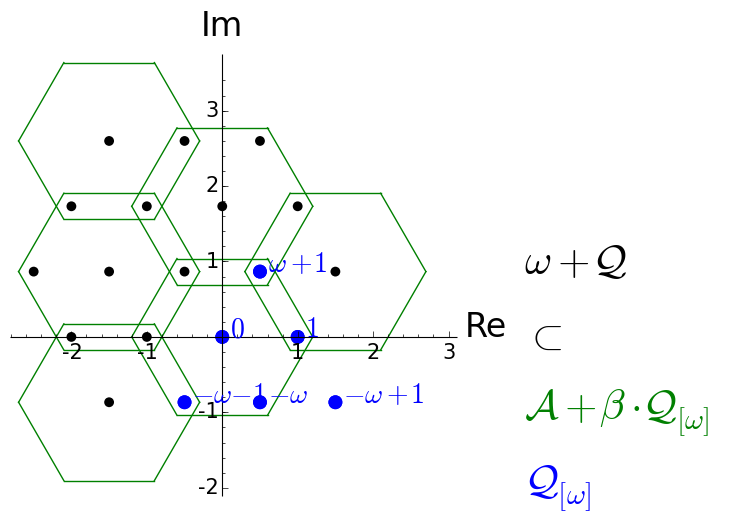
\includegraphics[width=0.2\textwidth]{img/phase2_image_3a.png}
    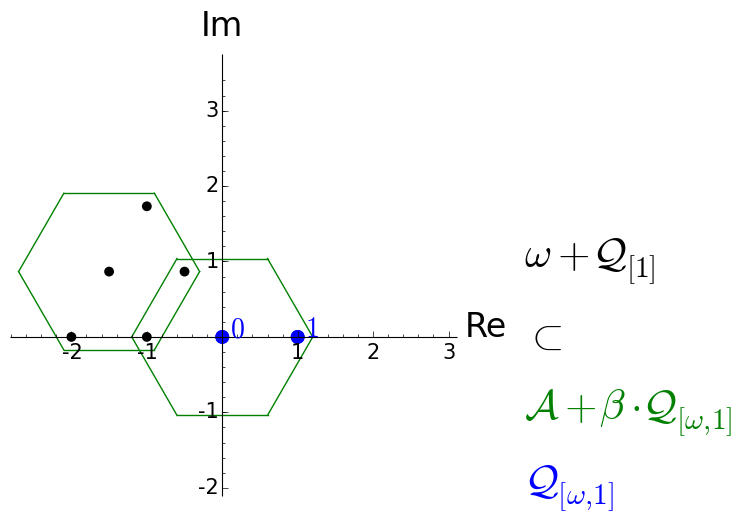
\includegraphics[width=0.2\textwidth]{img/phase2_image_5.png}
\end{tikzfigure}
Two steps of Phase 2 for input digits $\omega,1$.
}
\subcolumn{0.57}
\block{}{
  \begin{tikzfigure}[First iteration of Phase 1]
    %\centering
    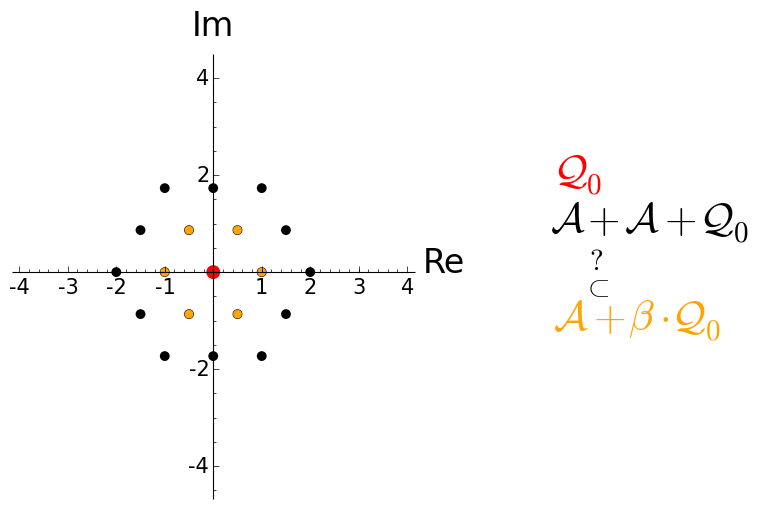
\includegraphics[width=0.2\textwidth]{img/phase1_image_3a.png}
    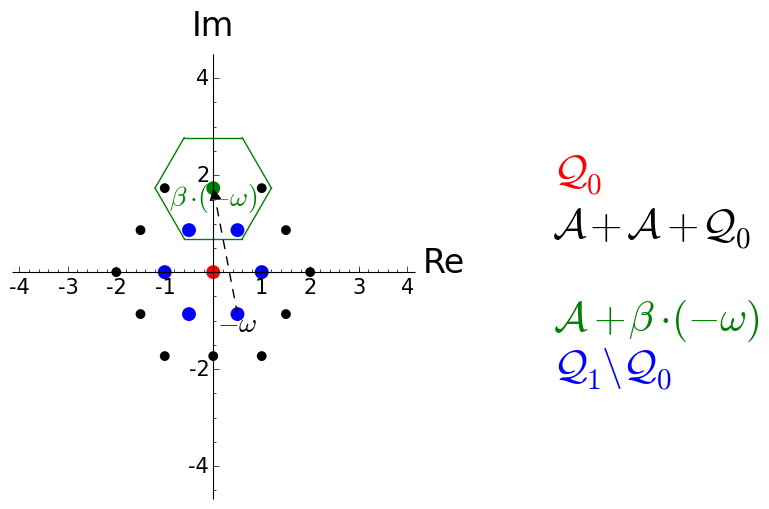
\includegraphics[width=0.2\textwidth]{img/phase1_image_4.png}
\end{tikzfigure}

\vspace{13pt}
}

\note[targetoffsetx=-.225\colwidth,targetoffsety=-0.09\colwidth,innersep=0.5cm,angle=-135, width=.6\subcolwidth]{Figures are plotted for Eisenstein base $$\beta = \omega -1\,,\omega=\imath\,\frac{1}{2} \sqrt{3}-\frac{1}{2}$$
%
%with the minimal polynomial $$m_\beta(x)=x^2+3x+3\,.$$
% 
and the alphabet $$\mathcal{A} =\{0, 1, -1, \omega, -\omega, -\omega - 1, \omega + 1\}$$}

\block{Phase 2}{
  \begin{algorithmic}[0]
 %   \FORALL{$w_j \in \A+\A$}
            \STATE For all $w_j \in \A+\A$, find set $\Q_{[w_{j}]} \subset \Q$ such that
              $$
              w_j + \underbrace{\Q}_{q_{j-1}\in} \subset \underbrace{\A}_{z_j\in} + \underbrace{\beta \Q_{[w_{j}]}}_{\beta q_j\in}\,.
              $$
             \vspace{-20pt}
%    \ENDFOR
    \STATE $k:=0$
    \WHILE{$\max\#\Qwo{k} > 1$}	%$\max\{\#\Qwo{k}:\tupleo{k} \in(\A+\A)^{k+1} \} > 1$
        \STATE $k:= k +1$
        %\FORALL{$\tupleo{k} \in (\A+\A)^{k+1}$}
            \STATE Find set $\Qwo{k} \subset \Qwo{(k-1)}$ such that
              $$
              w_j + \Qw{1}{k} \subset \A + \beta \Qwo{k}\,.
              $$%\vspace{-20pt}
              for all $\tupleo{k} \in (\A+\A)^{k+1}$.
        %\ENDFOR  
    \ENDWHILE  
    %\STATE $r:= k+1$ 
    %\STATE Define $q\tupleo{(r-1)}$ by only element of $\Qwo{(r-1)}$ for all $\tupleo{(r-1)}\in(\A+\A)^{r}$.
    \STATE Define $q\tupleo{k}$ by the only element of $\Qwo{k}$ for all $\tupleo{k}\in(\A+\A)^{k+1}$, $r:=k+1$.
%    \STATE 
%    \FORALL{$\tupleo{(r-1)}\in(\A+\A)^{r}$}
%	    \STATE $q\tupleo{(r-1)}:=$ only element of $\Qwo{(r-1)}$
%	\ENDFOR
  \end{algorithmic}
  \vspace{6pt}
}
\end{subcolumns}

\block{Convergence of Phase 1}{
	If the extending window method with the rewriting rule $x-\beta$ converges for the numeration system $(\beta, \A)$, then the base $\beta$ is expanding.

\vspace{20pt}

	Let $\A$ contain at least one representative of each congruence class modulo $\beta$ in $\Zomega$. If $\beta$ is expanding, then Phase 1 of the extending window method converges.
}

%\begin{subcolumns}
%\subcolumn{0.5}
%
%
%\subcolumn{0.5}
%
%
%\end{subcolumns}


\block{Non-convergence of Phase 2}{
If number of possible weight coefficients for input digits $bb\dots b$ does not decrease for some $b\in\A+\A$ when the length of window is increased, then Phase 2 does not converge.

\vspace{20pt}
If there is an infinite path in the graph which is defined by non-decreasing combinations, then Phase 2 does not converge.
}
\block{Examples}{
\centering
\begin{tabulary}{60cm}{C|CCC|CCC|C|CCC}
%$\omega$ & $\beta$ & $m_\beta$ & real conj. $>1$ &$\A\subset$& $\#\A$ & min. & $\#\Q$ & $bb\dots b$ & Phase 2 & $r$   \\ \midrule
%$ \frac{1}{2} i \, \sqrt{3} - \frac{1}{2} $ & $ \omega - 1 $ & $ x^{2} + 3 \, x + 3 $ & no &$\Zbeta$ & $ 7 $& yes & $ 19 $ & \checkmark & \checkmark & 3 \\ \midrule
$ i - 1 $ & $ \omega $ & $ x^{2} + 2 \, x + 2 $ & no & $\Zbeta$ &$ 5 $& yes & $ 45 $ & \checkmark & \checkmark & 6 \\ \midrule
$ -\frac{1}{2} \, \sqrt{21} + \frac{3}{2} $ & $ 2 \, \omega - 3 $ & $ x^{2} - 21 $ & yes & $\ZZ$ &$ 22 $& yes & $ 9 $ & \checkmark & \checkmark & 4 \\ \midrule
$ -\frac{1}{2} \, \sqrt{17} + \frac{3}{2} $ & $ 2 \, \omega - 3 $ & $ x^{2} - 17 $ & yes & $\ZZ$ &$ 19 $& no & $ 9 $ & \checkmark & \checkmark & 2 \\
$ -\frac{1}{2} \, \sqrt{17} + \frac{3}{2} $ & $ 2 \, \omega - 3 $ & $ x^{2} - 17 $ & yes &$\ZZ$& $ 18 $ & yes & $ 9 $ & \checkmark & \checkmark & 4 \\ \midrule
$ \frac{1}{2} i \, \sqrt{11} - \frac{3}{2} $ & $ \omega $ & $ x^{2} + 3 \, x + 5 $ & no & $\Zbeta$ &$ 9 $& yes & $ 11 $ & \checkmark & \xmark & - \\
$ \frac{1}{2} i \, \sqrt{11} - \frac{3}{2} $ & $ \omega $ & $ x^{2} + 3 \, x + 5 $ & no & $\Zbeta$ &$ 9 $& yes & $ 17 $ & \xmark & \xmark & - \\ \midrule
$ i \, \sqrt{2} - 1 $ & $ -\omega - 2 $ & $ x^{2} + 2 \, x + 3 $ & no &  $\Zbeta$ & $ 6 $ & yes  &$ 27 $& \checkmark & \checkmark & 7 \\
$ i \, \sqrt{2} - 1 $ & $ -\omega - 2 $ & $ x^{2} + 2 \, x + 3 $ & no & $\Zbeta$& $ 6 $ & yes  &$ 26 $& \checkmark & \xmark & - \\
\end{tabulary}

\vspace{6pt}
}


\block{}{
C.~Frougny, E.~Pelantov\'a, and M.~Svobodov\'a, \emph{Parallel addition in
  non-standard numeration systems}, Theoret. Comput. Sci. \textbf{412} (2011),
  5714--5727.

%C.~Frougny, E.~Pelantov{\'a}, and M.~Svobodov{\'a}, \emph{Minimal digit sets
%  for parallel addition in non-standard numeration systems}, J. Integer Seq.
%  \textbf{16} (2013), 36.
}


\end{columns}
%\center KM FJFI \v{C}VUT, Trojanova 13, 120 00 Praha 2, Czech Republic,  \url{jan.legersky@gmail.com}
\end{document}


